% Written by Richard Christopher, Copyright 2026 NeoTec Digital
\documentclass[11pt]{article}

\usepackage[T1]{fontenc}
\usepackage{lmodern}
\usepackage{amsmath}
\usepackage{amssymb}
\usepackage{graphicx}
\usepackage{booktabs}
\usepackage{float}
\usepackage{xcolor}
\usepackage[margin=1in]{geometry}
\usepackage[colorlinks=true,linkcolor=blue!45!black,citecolor=blue!45!black,urlcolor=blue!45!black]{hyperref}
\usepackage{microtype}

\DeclareMathOperator{\sgn}{sgn}
\DeclareMathOperator{\atantwo}{atan2}
\newcommand{\clamp}{\Pi}
\newcommand{\stvec}{\mathbf{s}}
\newcommand{\namedthm}[1]{\par\medskip\noindent\textbf{#1.}\ \itshape}
\newcommand{\qed}{\hfill$\square$}

% Final values, measured at seed 42 (N=4, T=2000).
\newcommand{\msFull}{0.113}
\newcommand{\msOpp}{0.000}
\newcommand{\msImit}{0.120}
\newcommand{\entFull}{0.622}
\newcommand{\entOpp}{0.131}
\newcommand{\entImit}{0.668}
\newcommand{\nvFull}{0.579}
\newcommand{\nvOpp}{0.501}
\newcommand{\nvImit}{0.261}

\title{Stable Chaos: Bounded Persistent Dynamics from Antagonistic and Imitative Coupling}
\author{Richard I. Christopher\\ \normalsize NeoTec Digital}
\date{2026}
\begin{document}
\maketitle

\begin{abstract}
Two coupling mechanisms pull a network of interacting units in opposite directions. Antagonistic (opposition)
coupling, acting alone, drives a system into a rigid, frozen, low-entropy configuration. Imitative (likeness)
coupling, acting alone, collapses the same system onto a single wandering consensus. We argue and demonstrate
computationally that combining the two yields dynamics that are simultaneously bounded and persistently
non-converging: trajectories never settle to a fixed point yet never diverge, and they occupy a large fraction of
the accessible state space. We adopt the established term \emph{stable chaos} of Politi and Torcini operationally to
name this regime. Two models make the claim concrete. The Stable Chaos Model (SCM) is a discrete-time ring of
two-channel nodes with a deterministic opposition rule and a stochastic imitation rule; ablating either mechanism
removes it, as opposition-only freezes and imitation-only herds. The Tranception lattice is a frustrated Kuramoto lattice whose couplings are signed by a
squared-distance orientation class, for which the $26$-site neighborhood decomposes exactly as $26=6+12+8$. We give
the model equations, the metrics used to quantify persistence and occupancy, an exact phasor superposition law that
corrects a legacy transform-domain implementation, and figures from deterministic seed-$42$ runs. The scope is a
model-level computational exploration; we make no continuum or hardware claims.
\end{abstract}

\section{Introduction}
\label{sec:intro}

Coupling between interacting units admits two elementary intuitions. \emph{Antagonistic} coupling---repulsion,
anti-alignment, or geometric frustration---tends to lock a system into a rigid, low-entropy arrangement, as in
antiferromagnetic order. \emph{Imitative} coupling---attraction, consensus, or phase alignment---tends to collapse
a population onto a single state that then drifts together, as in herding. Taken separately, neither mechanism
produces rich, sustained dynamics: one freezes and the other collapses. The thesis of this paper is that the two
mechanisms, acting together, produce dynamics that are at once \emph{bounded} and \emph{persistently
non-converging}. Opposition supplies the tension that prevents consensus; imitation supplies the mobility that
prevents freezing; their competition keeps the system exploring a large portion of its bounded state space
indefinitely.

We name this regime \emph{stable chaos}, borrowing the term from Politi and Torcini~\cite{politi2010}, who use it
for irregular dynamics that arise in systems that are linearly stable (non-positive maximal Lyapunov exponent) yet
exhibit long-lived aperiodic behavior. Our usage is deliberately operational rather than a claim about Lyapunov
spectra. We call a configuration operationally stable-chaotic when it satisfies two dynamical criteria on a compact
state space: (i) \emph{liveness}---the long-time mean step size stays bounded away from zero, so there is no fixed
point or short limit cycle; and (ii) \emph{diversity}---the units stay dispersed, with the cross-node variance held
well above zero rather than collapsing onto a single consensus. Boundedness is guaranteed by construction, and high
state-space occupancy follows from liveness together with diversity. The distinction matters: a single herd can
wander persistently and even visit a large fraction of the space over time, so occupancy alone does not separate
stable chaos from consensus drift---only the conjunction of liveness and cross-node diversity does. These are
model-level, computational criteria; we do not estimate Lyapunov exponents and make no continuum or hardware claims.

Two concrete models drive the paper. The Stable Chaos Model (SCM), Section~\ref{sec:scm}, is a discrete-time ring
of two-channel nodes formalizing a legacy prototype; it combines a deterministic opposition rule with a stochastic
imitation rule, and its two switches let us ablate each mechanism independently. The Tranception lattice,
Section~\ref{sec:lattice}, is a $d$-dimensional frustrated Kuramoto lattice whose couplings are signed by the
geometric orientation class of each neighbor pair. Section~\ref{sec:waves} contributes an exact phasor superposition
law used to correct a legacy transform-domain waveform implementation. Our contributions are: a symmetrized,
reproducible formalization of the SCM with quantitative occupancy and persistence metrics
(Sections~\ref{sec:scm}--\ref{sec:scmresults}); an orientation-class lattice with an exact neighborhood decomposition
and its frustrated phase dynamics (Sections~\ref{sec:lattice}--\ref{sec:latticeresults}); and a closed-form waveform
algebra (Section~\ref{sec:waves}). All figures are produced by deterministic runs seeded at $42$.

\section{The Stable Chaos Model}
\label{sec:scm}

\subsection{State space and topology}
The SCM is a ring of $N$ nodes with $N$ even and $N\ge 4$. Node $i\in\mathbb{Z}_N$ carries a state
$\stvec_i=(A_i,B_i)\in[-1,1]^2$; we call $A$ and $B$ its two channels. Three ring relations are used: the
\emph{opposite} $o(i)=(i+N/2)\bmod N$, the \emph{left} neighbor $\ell(i)=(i+1)\bmod N$, and the \emph{right}
neighbor $\rho(i)=(i-1)\bmod N$. The sign function is the three-valued
\begin{equation}
\sgn(x)=\begin{cases} -1, & x<0,\\ \phantom{-}0, & x=0,\\ +1, & x>0,\end{cases}
\end{equation}
and $\clamp(x)=\max(-1,\min(1,x))$ denotes clamping to $[-1,1]$, applied componentwise to a state. The update step
size is a fixed constant $\delta=0.0987$ inherited from the legacy prototype. Initial states are drawn
$A_i,B_i\sim\mathrm{Uniform}(-1,1)$ from a seeded generator, so every run is reproducible from its seed.

\subsection{Update rule}
The dynamics are synchronous: at tick $t$ all nodes read the configuration $\{\stvec_j(t)\}$ and write
$\{\stvec_j(t+1)\}$. Two increments act on each node, gated by boolean switches $\mathbb{1}_{\mathrm{opp}}$ and
$\mathbb{1}_{\mathrm{imit}}$.

The \emph{opposition} increment encodes the legacy repulsion semantics, in which the $A$-channel opposes the
opposite node while the $B$-channel follows it:
\begin{equation}
\Delta^{\mathrm{O}}_i(t)=\Bigl(\delta\,\sgn\!\left(A_i-A_{o(i)}\right),\;
\sgn\!\left(B_{o(i)}-B_i\right)\,\min\!\bigl(\delta,\;\tfrac12\lvert B_{o(i)}-B_i\rvert\bigr)\Bigr).
\label{eq:opp}
\end{equation}
The $B$-channel follows to consensus, but its step is capped at half the gap $\lvert B_{o(i)}-B_i\rvert$. This cap is
essential to the freeze result. A pure sign-step follow, $\delta\,\sgn(B_{o(i)}-B_i)$, never reaches a fixed point:
a mutually following pair overshoots the meeting point every tick and settles into a permanent $\pm\delta$ limit
cycle about it, a discretization artifact rather than genuine motion. Capping the step at half the gap lets a
diametric pair meet exactly at its midpoint and rest there, which is what makes the opposition-only model \emph{truly}
freeze instead of jitter. The cap is inactive when the pair is far apart---it coincides with $\delta\,\sgn(B_{o(i)}-B_i)$
whenever $\lvert B_{o(i)}-B_i\rvert>2\delta$. Acting alone this increment is deterministic: the $A$-channels amplify
their differences until they saturate at $\pm1$, while the $B$-channels are pulled together and rest, so the
configuration relaxes onto a rigid, low-mobility arrangement.

The \emph{imitation} increment is stochastic. At each node draw two independent variates
$r_A,r_B\sim\mathrm{Uniform}\{-1,0,+1\}$ and set
\begin{equation}
\Delta^{\mathrm{I}}_i(t)=
\begin{cases}
\delta\,(-1,-1), & (r_A,r_B)=(+1,+1),\\[2pt]
\delta\,(+1,+1), & (r_A,r_B)=(-1,-1),\\[2pt]
\delta\,r_A\bigl(\sgn(A_{\ell(i)}-A_i),\,\sgn(B_{\ell(i)}-B_i)\bigr), & r_A\neq 0\ \text{(else)},\\[2pt]
\delta\,r_B\bigl(\sgn(A_{\rho(i)}-A_i),\,\sgn(B_{\rho(i)}-B_i)\bigr), & r_A=0,\ r_B\neq 0,\\[2pt]
(0,0), & r_A=r_B=0.
\end{cases}
\label{eq:imit}
\end{equation}
The first two cases are joint retreat and joint advance along the state diagonal. Otherwise the node moves toward
($+1$) or away from ($-1$) its left neighbor when $r_A\neq0$, or its right neighbor when only $r_B\neq0$; the
coefficient $r_A$ (resp.\ $r_B$) flips ``toward'' into ``away.'' Acting alone this is a stochastic consensus drift:
nodes chase and flee their ring neighbors, wandering without the tension needed to keep exploring.

The full synchronous update is \emph{sequential}: the opposition increment is applied first to form a clamped
working self $\mathbf{w}_i$, and the imitation increment then acts on that working self, while every \emph{neighbor}
state is still read from the tick-$t$ configuration:
\begin{equation}
\begin{aligned}
\mathbf{w}_i &= \clamp\!\left[\stvec_i(t)+\mathbb{1}_{\mathrm{opp}}\,\Delta^{\mathrm{O}}_i\!\bigl(\stvec(t)\bigr)\right],\\[2pt]
\stvec_i(t+1) &= \clamp\!\left[\mathbf{w}_i+\mathbb{1}_{\mathrm{imit}}\,\Delta^{\mathrm{I}}_i\!\bigl(\mathbf{w}_i,\stvec(t)\bigr)\right].
\end{aligned}
\label{eq:update}
\end{equation}
Here $\Delta^{\mathrm{O}}_i$ is evaluated entirely at $\stvec(t)$, whereas in $\Delta^{\mathrm{I}}_i$ the node's own
references $A_i,B_i$ of Equation~\eqref{eq:imit} are taken at the working self $\mathbf{w}_i$ while the neighbor
references $A_{\ell(i)},B_{\ell(i)},A_{\rho(i)},B_{\rho(i)}$ remain at tick $t$; imitation's toward/away sign is
therefore measured against the post-opposition working self, not against $\stvec_i(t)$. The clamp $\clamp$ is applied
at each sub-step, so an intermediate excursion past $[-1,1]$ is never carried into the next term. Because both
increments read all neighbors synchronously at tick $t$ and are applied to every node in the same fixed order, the
update is independent of node iteration order.
The legacy four-node prototype applied heterogeneous, iteration-order-dependent rules;
Equations~\eqref{eq:opp}--\eqref{eq:update} are their symmetrized, order-independent formalization (the per-node
quirks are documented separately in the repository legacy notes).

\subsection{Ablations}
Equation~\eqref{eq:update} defines three variants through the switches. The \emph{full} model runs both increments
($\mathbb{1}_{\mathrm{opp}}=\mathbb{1}_{\mathrm{imit}}=1$). The \emph{opposition-only} model keeps only
$\Delta^{\mathrm{O}}$ and is deterministic. The \emph{imitation-only} model keeps only $\Delta^{\mathrm{I}}$ and is
purely stochastic. These three variants are the empirical basis for the thesis: only the full model is expected to
remain both persistently mobile and dispersed across $[-1,1]^2$, whereas opposition-only freezes and imitation-only
herds into a single cluster.

\subsection{Metrics}
\label{sec:metrics}
A trajectory is stored as an array of shape $(T,N,2)$. We quantify it with the following scalars, defined here
exactly as they are computed. For a configuration at tick $t$ write $\chi_i(t)$ for channel $\chi\in\{A,B\}$ of node
$i$ and $\bar\chi(t)=\tfrac1N\sum_i\chi_i(t)$.

The per-tick \emph{node variance}, averaged over channels, measures cross-node dispersion:
\begin{equation}
V(t)=\frac{1}{2}\sum_{\chi\in\{A,B\}}\frac1N\sum_{i}\bigl(\chi_i(t)-\bar\chi(t)\bigr)^2.
\end{equation}
The \emph{mean step size}, the mean Euclidean per-node displacement over the final $w$ transitions, measures
persistence; values near zero indicate a frozen state:
\begin{equation}
S_w=\frac{1}{wN}\sum_{t=T-w}^{\,T-1}\sum_{i}\bigl\lVert\stvec_i(t+1)-\stvec_i(t)\bigr\rVert_2.
\end{equation}
The \emph{occupancy entropy} bins the pooled $(A,B)$ samples over all nodes and ticks into a $b\times b$ grid on
$[-1,1]^2$, forms the empirical distribution $p_k=n_k/\sum_k n_k$, and normalizes the Shannon entropy (in nats) by
$\ln b^2$ so that $\hat H\in[0,1]$:
\begin{equation}
\hat H=\frac{-\sum_{k:\,p_k>0}p_k\ln p_k}{\ln b^2}.
\label{eq:entropy}
\end{equation}
For a one-dimensional series $x_t$ the normalized \emph{autocorrelation} at lag $k$ is
\begin{equation}
\rho(k)=\frac{\sum_t (x_t-\bar x)(x_{t+k}-\bar x)}{\sum_t (x_t-\bar x)^2},\qquad \rho(0)=1.
\end{equation}
Two aggregates carry over to the phase models. The \emph{Kuramoto order parameter} of $N$ phases $\varphi_j$ is
\begin{equation}
r=\Bigl|\tfrac1N\sum_{j}e^{i\varphi_j}\Bigr|\in[0,1],
\label{eq:kuramoto}
\end{equation}
and the \emph{acumen}, the legacy global aggregate, is the mean state $\bar\stvec=\tfrac1N\sum_i\stvec_i\in
\mathbb{R}^2$.

\section{SCM Results}
\label{sec:scmresults}

All SCM figures use $N=4$, $T=2000$ ticks, and seed $42$. Figure~\ref{fig:traj} plots the two channels of every
node over time. The full model produces channels that keep moving throughout the run without collapsing to a
constant or to a short cycle, the visual signature of persistence. Figure~\ref{fig:portrait} shows the same run as
$(A,B)$ paths per node with start and end markers; the nodes migrate to the two vertical edges $A=\pm1$ and then
keep sweeping in $B$ along them, rather than parking at a single corner or converging to a common point.

\begin{figure}[H]
\centering
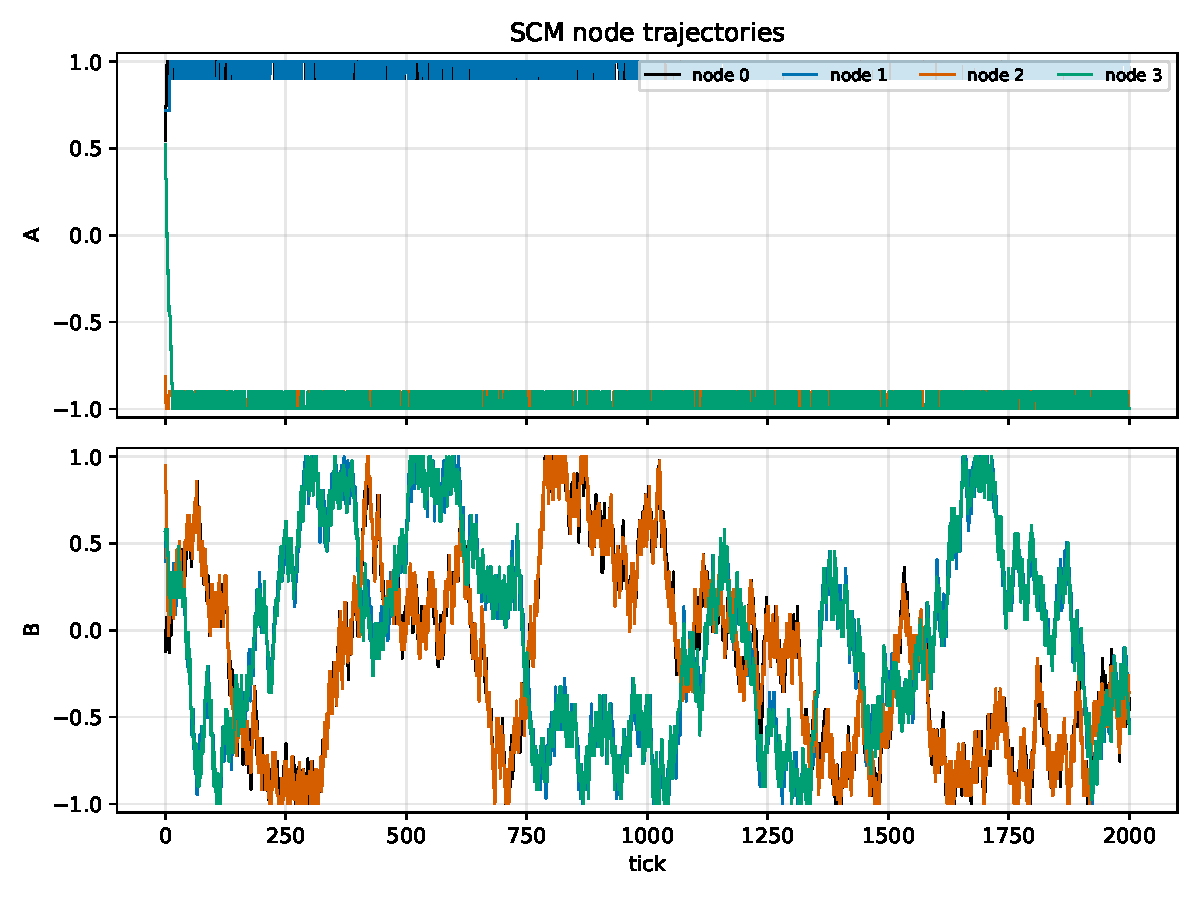
\includegraphics[width=0.9\linewidth]{figures/fig_scm_trajectories.pdf}
\caption{SCM channel trajectories $A_i(t)$ (top) and $B_i(t)$ (bottom) for the full model, $N=4$, seed $42$.
Channels remain active for the full run rather than settling.}
\label{fig:traj}
\end{figure}

\begin{figure}[H]
\centering
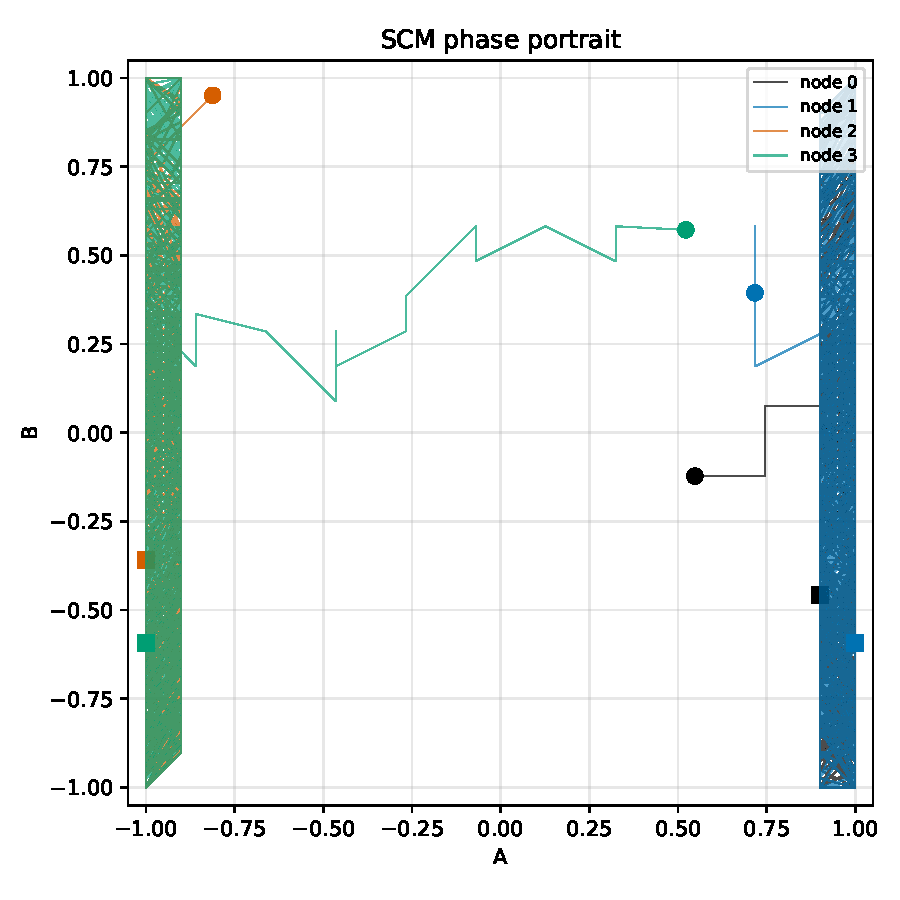
\includegraphics[width=0.72\linewidth]{figures/fig_scm_phase_portrait.pdf}
\caption{Phase portrait: per-node paths in the $(A,B)$ plane with start (open) and end (filled) markers. The nodes
settle onto the two vertical bands $A=\pm1$ while continuing to wander in $B$, rather than converging to a single
fixed point.}
\label{fig:portrait}
\end{figure}

The ablation, Figure~\ref{fig:ablation}, contrasts the three variants directly. The opposition-only model relaxes
to a rigid configuration: its late-time mean step size falls to zero and it freezes, yet its nodes remain
dispersed---the antagonistic $A$-channels saturate against opposite clamps, so the cross-node variance stays high
while nothing moves. The imitation-only model is the mirror image: it stays mobile but herds, so its cross-node
variance collapses as the nodes chase one another into a common wandering cluster. The full model is the only
variant that is simultaneously live and dispersed. Figure~\ref{fig:occupancy} shows the pooled two-dimensional
occupancy of the full model: two high-count bands at $A=\pm1$ with the $B$-channel sweeping the full range $[-1,1]$
inside them---frozen antagonistic order in $A$ coexisting with persistent wandering in $B$.

\begin{figure}[H]
\centering
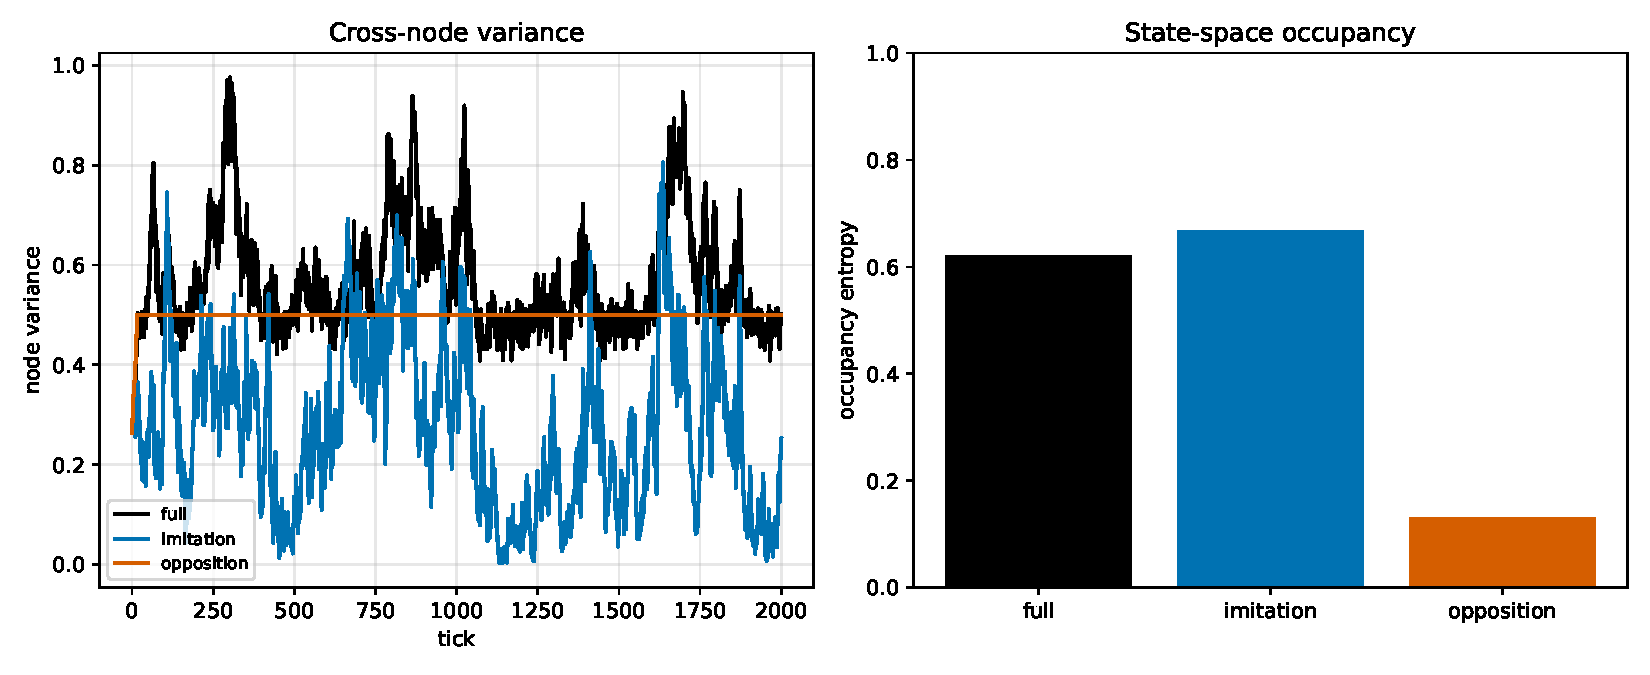
\includegraphics[width=0.95\linewidth]{figures/fig_scm_ablation.pdf}
\caption{Ablation. Left: node variance $V(t)$ for the full, opposition-only, and imitation-only variants. Right:
normalized occupancy entropy $\hat H$ per variant. Opposition-only freezes (variance stays high but nothing moves);
imitation-only in fact reaches the \emph{highest} occupancy entropy, but as a consensus herd whose cross-node variance
collapses (left panel); the full model pairs comparable entropy with sustained cross-node diversity.}
\label{fig:ablation}
\end{figure}

\begin{figure}[H]
\centering
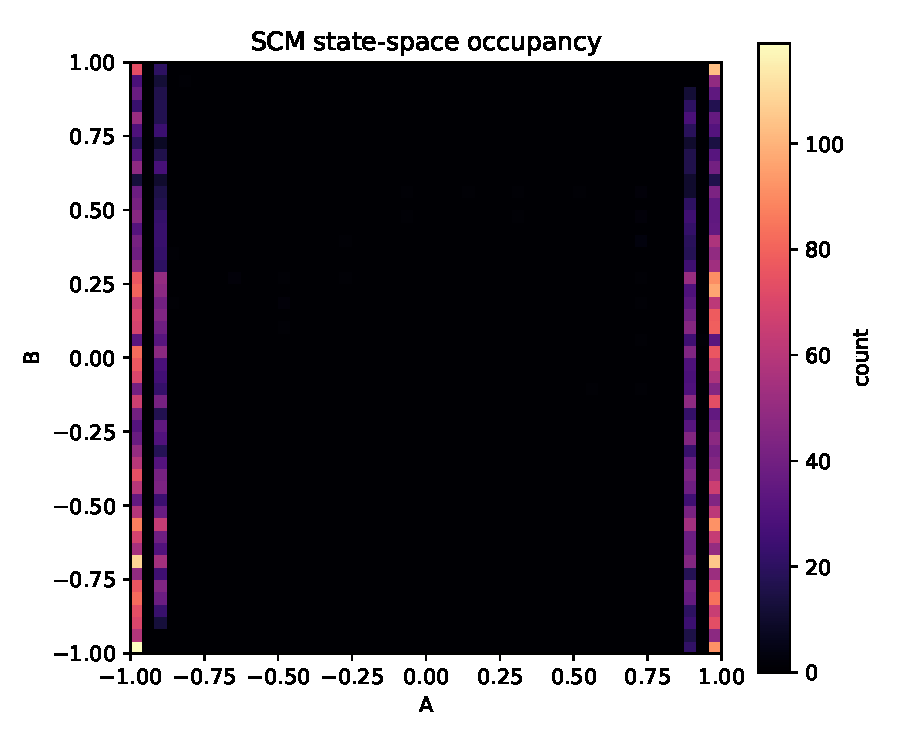
\includegraphics[width=0.62\linewidth]{figures/fig_scm_occupancy.pdf}
\caption{Pooled occupancy histogram of the full model over all nodes and ticks. Occupancy concentrates in two
vertical bands at $A=\pm1$---the antagonistic $A$-channel pins to the clamps---while the $B$-channel sweeps the full
range $[-1,1]$ within them. The high normalized entropy of Equation~\eqref{eq:entropy} ($\hat H=\entFull$) comes from
this $B$-spread inside the two bands, not from broad interior coverage: frozen order in $A$ coexisting with persistent
wandering in $B$.}
\label{fig:occupancy}
\end{figure}

Table~\ref{tab:scm} reports the three summary scalars for each variant from the seed-$42$ runs, and they tell a
more careful story than occupancy alone would. Occupancy entropy separates only the frozen opposition-only variant
($\hat H=\entOpp$) from the two live variants; between those two it does \emph{not} favor the full model. The
imitation-only herd in fact wanders through slightly \emph{more} of the state space over time ($\hat H=\entImit$
versus $\entFull$ for the full model), because, being unanchored, its consensus cluster drifts freely across the
square. What distinguishes the variants is the \emph{conjunction} of two criteria. The first is liveness, the
late-time mean step size: it is $\msFull$ for the full model and $\msImit$ for imitation-only, but $\msOpp$ for
opposition-only, which is frozen. The second is diversity, the cross-node variance over the last $500$ ticks: it is
$\nvFull$ for the full model but collapses to $\nvImit$ for the imitation-only herd, while opposition-only stays
dispersed at $\nvOpp$ because its $A$-channels are pinned at opposite clamps. Opposition-only thus fails liveness,
imitation-only fails diversity, and only the full model satisfies both---persistent motion together with sustained
cross-node spread. We restrict quantitative claims to Table~\ref{tab:scm} and to this two-criteria separation; all
other claims are the qualitative ones the figures make directly.

\begin{table}[H]
\centering
\caption{SCM summary metrics, seed $42$, $N=4$, $T=2000$. Mean step size $S_w$ over the final $w=200$ transitions;
occupancy entropy $\hat H$ with $b=16$ bins, normalized to $[0,1]$; cross-node variance $\overline{V}$ time-averaged
over the final $500$ ticks.}
\label{tab:scm}
\begin{tabular}{lccc}
\toprule
Variant & \shortstack{Mean step\\ size $S_{200}$} & \shortstack{Occupancy\\ entropy $\hat H$}
        & \shortstack{Cross-node variance\\ $\overline{V}$ (last 500)} \\
\midrule
Full (opposition $+$ imitation) & \msFull & \entFull & \nvFull \\
Opposition only                 & \msOpp  & \entOpp  & \nvOpp  \\
Imitation only                  & \msImit & \entImit & \nvImit \\
\bottomrule
\end{tabular}
\end{table}

\section{The Tranception Lattice}
\label{sec:lattice}

\subsection{Orientation classes}
The second model places phase oscillators on a $d$-dimensional cubic lattice, $d\in\{1,2,3\}$, of side $L$, with
$L^d$ nodes indexed $0,\dots,L^d-1$ and integer coordinates recovered by the usual mixed-radix map. Each node is
embedded in $\mathbb{Z}^3$ by padding absent axes with zeros so that a single classifier serves every dimension. For
a coordinate offset $\mathbf{c}=(c_x,c_y,c_z)\in\{-1,0,+1\}^3$ we classify the neighbor pair by squared Euclidean
distance $\|\mathbf{c}\|^2=c_x^2+c_y^2+c_z^2$:
\begin{equation}
\text{class}(\mathbf{c})=
\begin{cases}
\textsc{self}, & \|\mathbf{c}\|^2=0,\\
\textsc{orthogonal}, & \|\mathbf{c}\|^2=1,\\
\textsc{adjacent}, & \|\mathbf{c}\|^2=2,\\
\textsc{polar}, & \|\mathbf{c}\|^2=3,
\end{cases}
\end{equation}
and the classifier is undefined (no coupling) whenever any $|c_k|>1$ or $\|\mathbf{c}\|^2>3$, i.e.\ outside the
$27$-site cube. Couplings are stored as unique undirected pairs with the \textsc{self} class excluded; on a torus
(the \texttt{toroidal} option) coordinates wrap modulo $L$. The following exact decomposition motivates the naming.

\namedthm{Proposition 1 (Neighborhood decomposition)}
The $26$ non-central sites of the cube $\{-1,0,+1\}^3$ split by orientation class as
\begin{equation}
26=\underbrace{6}_{\textsc{orthogonal}}+\underbrace{12}_{\textsc{adjacent}}+\underbrace{8}_{\textsc{polar}}.
\end{equation}
\upshape
\namedthm{Proof}
\upshape
Because each $c_k\in\{-1,0,+1\}$ we have $c_k^2\in\{0,1\}$, so $\|\mathbf{c}\|^2$ equals the number $m$ of nonzero
coordinates. Sites at squared distance $m$ are those with exactly $m$ nonzero coordinates, each chosen as $\pm1$:
there are $\binom{3}{m}2^m$ of them. Thus $m=1$ gives $\binom{3}{1}2=6$, $m=2$ gives $\binom{3}{2}2^2=12$, and $m=3$
gives $\binom{3}{3}2^3=8$, summing to $26$. \qed

\medskip
An interior node of a three-dimensional lattice therefore has exactly $6$ orthogonal, $12$ adjacent, and $8$ polar
neighbors; Figure~\ref{fig:neighborhood} renders the three classes. Corner and edge nodes on a non-toroidal lattice
have fewer, while on a torus every node recovers the full $6/12/8$ split.

\begin{figure}[H]
\centering
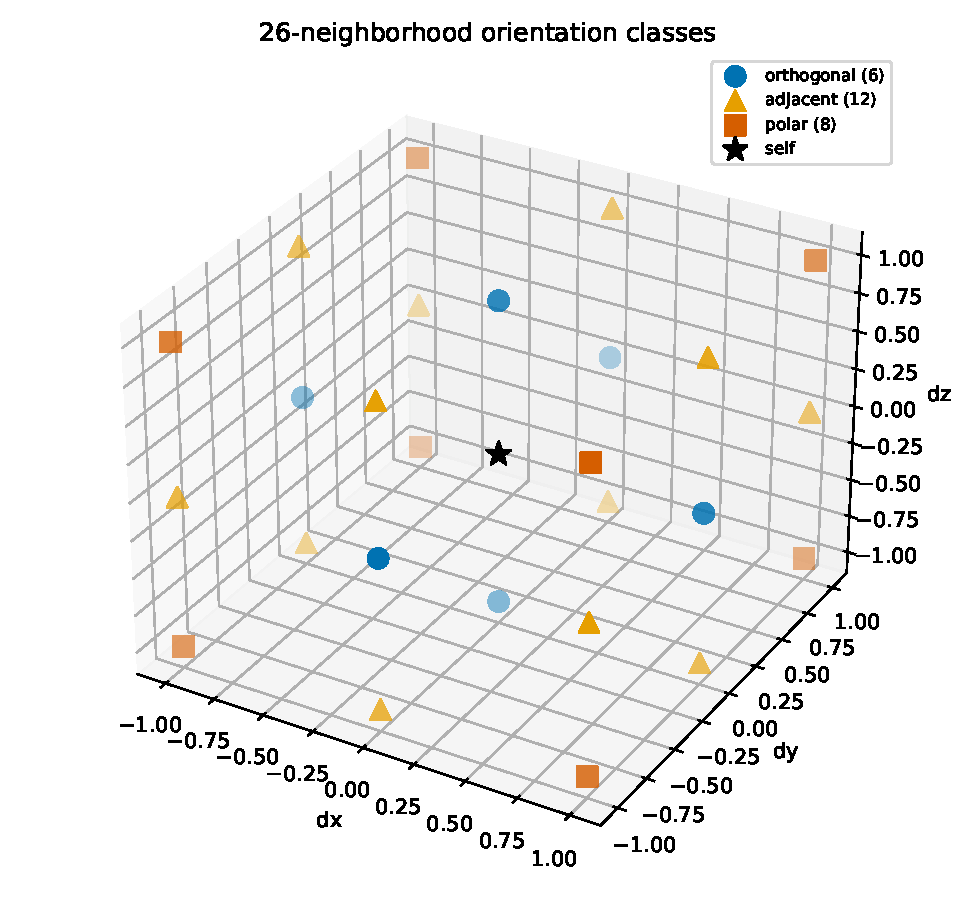
\includegraphics[width=0.6\linewidth]{figures/fig_neighborhood.pdf}
\caption{The $26$-site neighborhood of Proposition~1, colored by orientation class: $6$ orthogonal (face), $12$
adjacent (edge), and $8$ polar (corner) neighbors of the central node.}
\label{fig:neighborhood}
\end{figure}

\subsection{Signed phase dynamics}
Each node $i$ carries a phase $\varphi_i\in[0,2\pi)$ initialized uniformly, and a natural frequency
$\omega_i\sim\mathcal{N}(\mu,\sigma^2)$. Each orientation class $c$ is assigned a coupling constant $K_c$, with the
polar class taken negative to introduce frustration. Writing $N_c(i)$ for the class-$c$ neighbors of $i$, the
mean-field-normalized dynamics are the frustrated Kuramoto lattice
\begin{equation}
\dot\varphi_i=\omega_i+\sum_{c}\frac{K_c}{|N_c(i)|}\sum_{j\in N_c(i)}\sin(\varphi_j-\varphi_i),
\label{eq:phaseode}
\end{equation}
where classes with $|N_c(i)|=0$ contribute no term. The per-class normalization makes the drive comparable across
nodes of different degree. We integrate Equation~\eqref{eq:phaseode} with a forward Euler step of size $\Delta t$
and wrap onto the circle,
\begin{equation}
\varphi_i(t+\Delta t)=\Bigl[\varphi_i(t)+\Delta t\,\dot\varphi_i(t)\Bigr]\bmod 2\pi,
\end{equation}
and read out global coherence with the Kuramoto order parameter $r$ of Equation~\eqref{eq:kuramoto}. With
$K_{\mathrm{orth}}>0$ and $K_{\mathrm{adj}}>0$ the orthogonal and adjacent classes favor alignment; the negative
polar coupling $K_{\mathrm{polar}}<0$ opposes it, and the balance between the two is what the next section sweeps.

\section{Lattice Results}
\label{sec:latticeresults}

We integrate a $6\times6\times6$ toroidal lattice ($d=3$) for $4000$ steps at $\Delta t=0.05$ with
$K_{\mathrm{orth}}=1$, $K_{\mathrm{adj}}=0.5$, and varying polar coupling, all seeded at $42$; the experiments use a
genuinely three-dimensional lattice because the polar orientation class is empty in lower dimensions, as the Remark
below makes precise. Figure~\ref{fig:order} tracks the order parameter $r(t)$ for $K_{\mathrm{polar}}\in\{0,-0.5,-1\}$.
Without frustration ($K_{\mathrm{polar}}=0$) the alignment terms dominate and $r$ climbs to near-total coherence,
$r\approx0.996$: the lattice synchronizes. Switching on the polar coupling collapses coherence: at
$K_{\mathrm{polar}}=-1$ the frustration overwhelms alignment and the time-averaged order parameter falls to
$r\approx0.004$, an essentially incoherent field. The intermediate coupling $K_{\mathrm{polar}}=-0.5$ still
synchronizes, only more slowly, plateauing near $r\approx0.98$; the transition to incoherence sits between $-0.5$ and
$-0.75$ in the sweep of Figure~\ref{fig:sweep}.

\namedthm{Remark (Dimensional threshold)}\upshape
Polar frustration is intrinsically three-dimensional in this framework. A polar neighbor is a site at squared
distance three, which requires three simultaneously nonzero coordinates; in one or two dimensions no such offset
exists, so the polar class is empty and $K_{\mathrm{polar}}$ multiplies an absent term. The frustration is therefore
\emph{vacuous} below three dimensions: on a lattice with $d\le2$ the polar coupling has no effect whatsoever. We
confirmed this with a two-dimensional control, a $12\times12$ torus under otherwise identical settings, whose
time-averaged order parameter is identical to four decimals with and without polar coupling ($r=0.9905$ for both
$K_{\mathrm{polar}}=0$ and $K_{\mathrm{polar}}=-1$). This is why the sweep and order experiments use a three-dimensional
lattice, where the eight polar corners are present and can frustrate the six orthogonal and twelve adjacent
alignment bonds.

\begin{figure}[H]
\centering
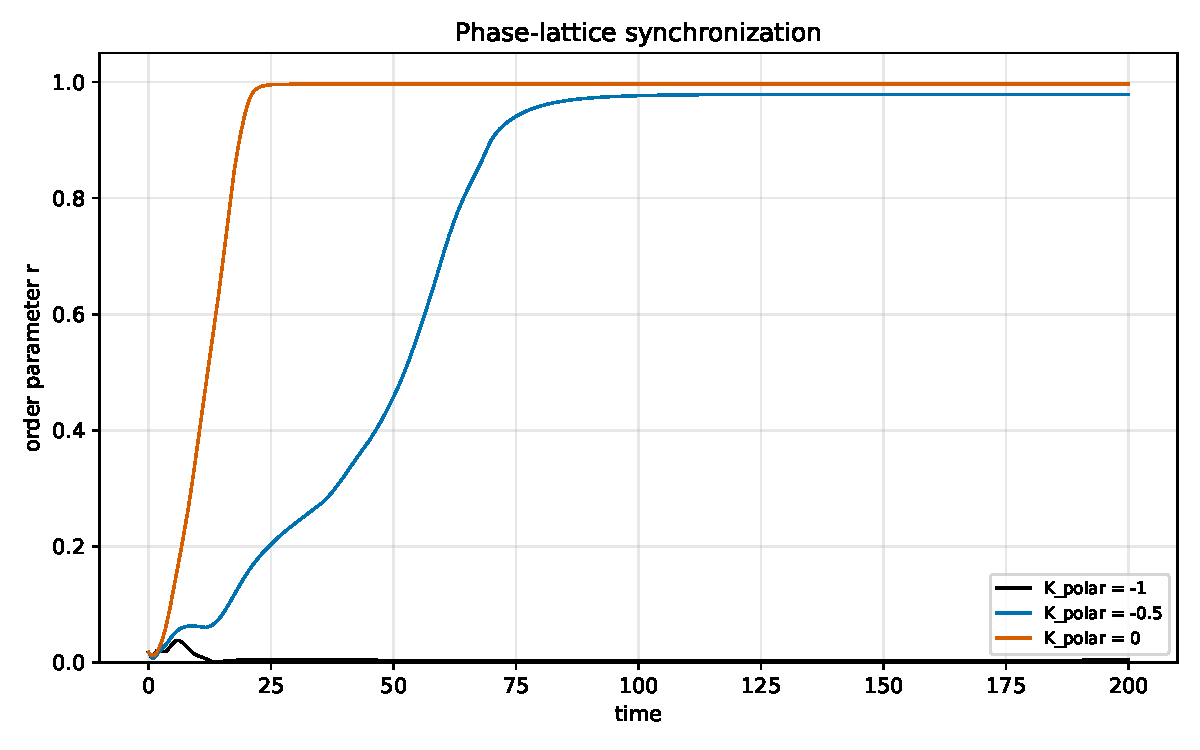
\includegraphics[width=0.85\linewidth]{figures/fig_lattice_order.pdf}
\caption{Order parameter $r(t)$ on a $6\times6\times6$ torus for three polar couplings. Unfrustrated coupling
($K_{\mathrm{polar}}=0$) synchronizes ($r\approx0.996$); strong frustration ($K_{\mathrm{polar}}=-1$) collapses
coherence ($r\approx0.004$).}
\label{fig:order}
\end{figure}

Figure~\ref{fig:sweep} sweeps $K_{\mathrm{polar}}$ across $\mathrm{linspace}(-2,0.5,11)$ and reports the
time-averaged $\langle r\rangle$ over the last quarter of each run. Coherence is high for non-negative polar
coupling and is sharply suppressed as $K_{\mathrm{polar}}$ becomes more negative, tracing the transition from
synchronization to a frustrated, incoherent regime. Figure~\ref{fig:phases} contrasts the two regimes directly
through the middle $z$-slice of the $6\times6\times6$ torus after $4000$ steps: the synchronized field
($K_{\mathrm{polar}}=0$, left) is nearly a single hue, whereas the frustrated field ($K_{\mathrm{polar}}=-1$, right) is
a disordered patchwork of phases, the spatial signature of the collapse in coherence.

\begin{figure}[H]
\centering
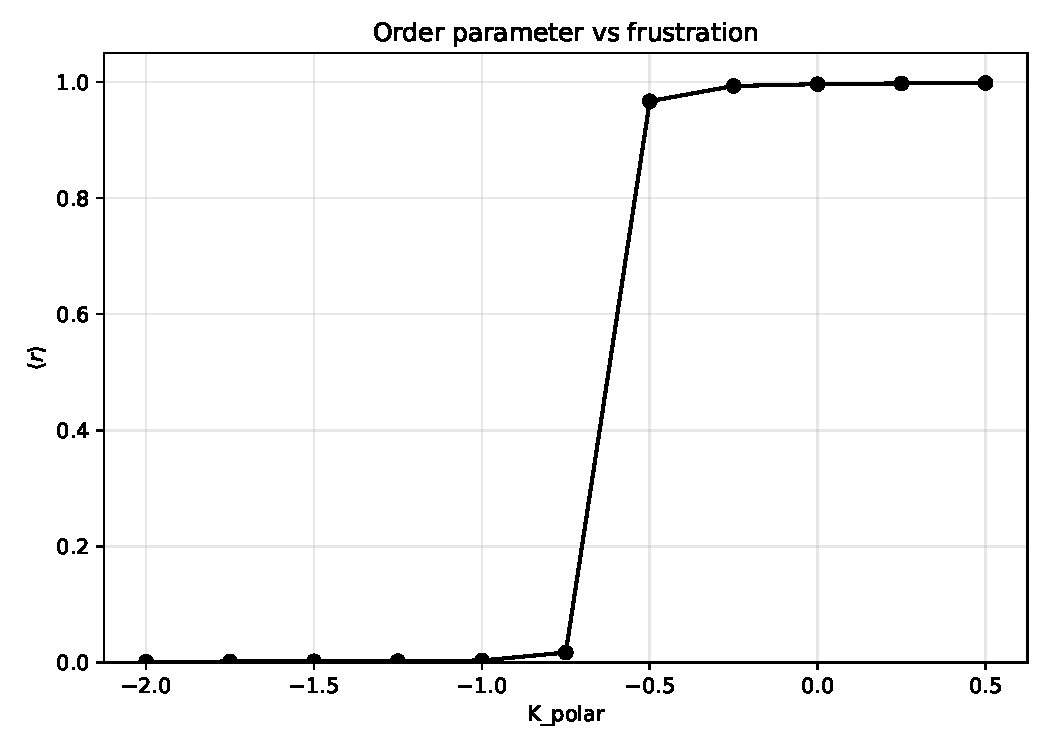
\includegraphics[width=0.72\linewidth]{figures/fig_lattice_sweep.pdf}
\caption{Time-averaged order parameter $\langle r\rangle$ versus polar coupling $K_{\mathrm{polar}}$ on the
$6\times6\times6$ torus. Synchronization is suppressed as frustration increases.}
\label{fig:sweep}
\end{figure}

\begin{figure}[H]
\centering
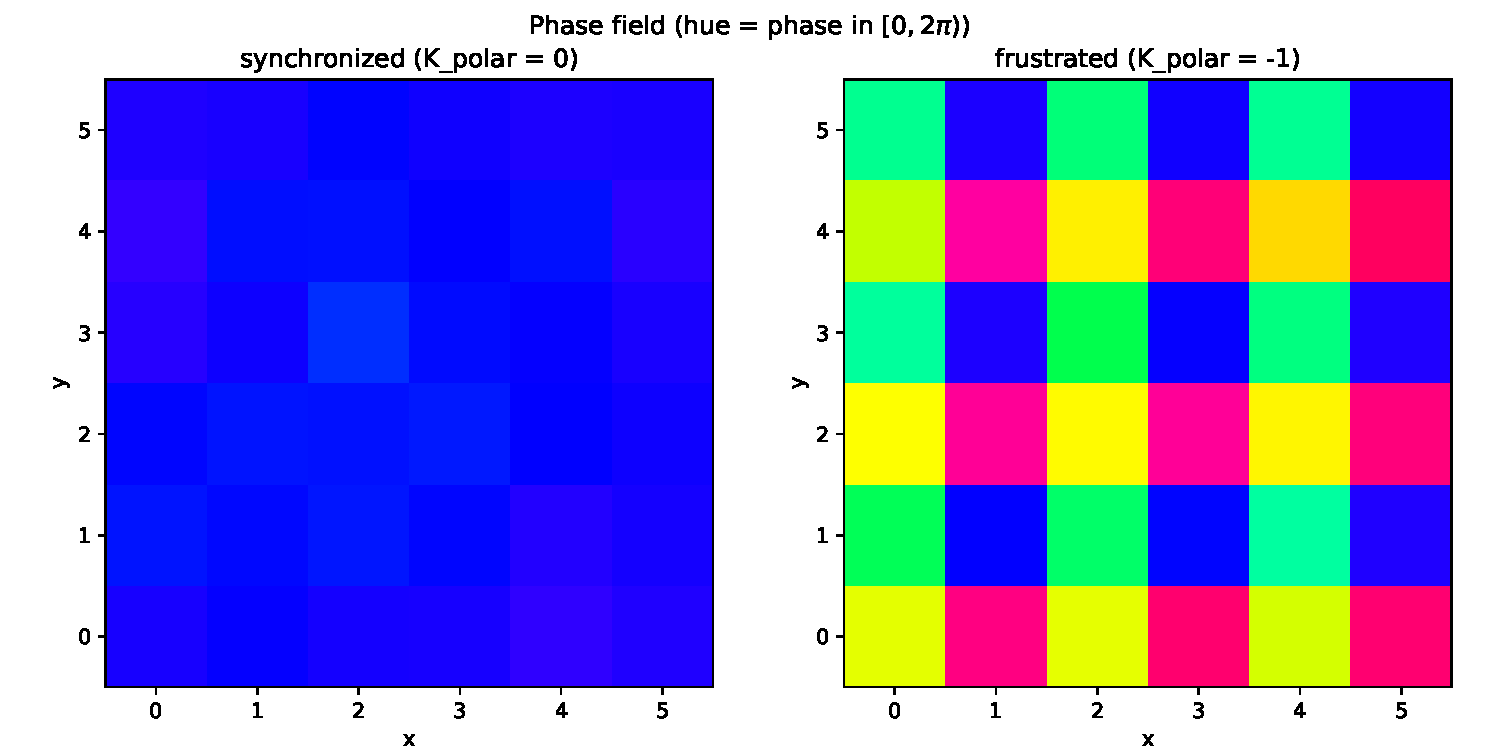
\includegraphics[width=0.55\linewidth]{figures/fig_lattice_phases.pdf}
\caption{Middle $z$-slice of the $6\times6\times6$ toroidal phase field after $4000$ steps, colored by phase. Left:
synchronized regime ($K_{\mathrm{polar}}=0$), a near-uniform hue. Right: frustrated regime ($K_{\mathrm{polar}}=-1$), a
disordered patchwork consistent with $r\approx0.004$.}
\label{fig:phases}
\end{figure}

The two models thus tell the same story with different vocabularies. In the SCM the deterministic opposition rule
freezes and the stochastic imitation rule herds, while their combination stays both mobile and diverse. In the lattice,
alignment couplings synchronize and the negative polar coupling frustrates, while their combination holds the field
in a partially ordered, non-uniform state. Antagonism and imitation are again in tension, and the tension is what
sustains the dynamics.

\section{Waveform Algebra}
\label{sec:waves}

The legacy Tranception code combined waveforms by transforming sampled buffers to the frequency domain, adding, and
transforming back. That round trip is exact only up to sampling and truncation error and leaks energy across
frequency bins. For sinusoids of a common frequency the correct combination is closed-form and exact, given by
phasor addition.

\namedthm{Lemma 1 (Phasor superposition)}
For two sinusoids of common frequency $f$, $y_k(t)=a_k\sin(2\pi f t+\phi_k)$ with $a_k\ge 0$, the sum is a single
sinusoid of the same frequency,
\begin{equation}
y_1(t)+y_2(t)=a_3\sin(2\pi f t+\phi_3),
\end{equation}
\upshape
whose amplitude and phase are those of the complex phasor sum $a_1e^{i\phi_1}+a_2e^{i\phi_2}=a_3e^{i\phi_3}$:
\begin{align}
a_3&=\sqrt{a_1^2+a_2^2+2a_1a_2\cos(\phi_1-\phi_2)},\\
\phi_3&=\atantwo\!\bigl(a_1\sin\phi_1+a_2\sin\phi_2,\;a_1\cos\phi_1+a_2\cos\phi_2\bigr).
\end{align}
Subtraction replaces $a_2e^{i\phi_2}$ by $-a_2e^{i\phi_2}$, equivalently $\phi_2\mapsto\phi_2+\pi$.

\namedthm{Proof}
\upshape
Write $\theta=2\pi f t$ and use $\sin\alpha=\operatorname{Im}e^{i\alpha}$. Then
$y_1+y_2=\operatorname{Im}\!\bigl(e^{i\theta}(a_1e^{i\phi_1}+a_2e^{i\phi_2})\bigr)
=\operatorname{Im}\!\bigl(e^{i\theta}a_3e^{i\phi_3}\bigr)=a_3\sin(\theta+\phi_3)$. The modulus and argument of the
phasor sum give $a_3$ and $\phi_3$; the modulus expands to the stated law by the cosine rule. \qed

\medskip
The implementation follows the lemma. Same-frequency addition and subtraction use the phasor law exactly, and a
frequency mismatch is rejected with an explicit error rather than silently approximated. Multiplication keeps the
legacy convention---product of amplitudes and sum of phases---which is a design choice rather than the trigonometric
product-to-sum identity, and it is documented as such. The resonant frequency of two waveforms is $f$ when they
agree and the geometric mean $\sqrt{f_1 f_2}$ otherwise; the reception level is $a_1a_2$ at equal frequency and zero
otherwise, preserving legacy semantics. Waveforms of arbitrary, possibly distinct frequencies are combined by
\texttt{superpose}, which sums samples directly in the time domain; the resulting amplitude never exceeds the sum of
the parts. Figure~\ref{fig:wave} shows two components and their superposition, including the beat envelope that
arises when their frequencies are close.

\begin{figure}[H]
\centering
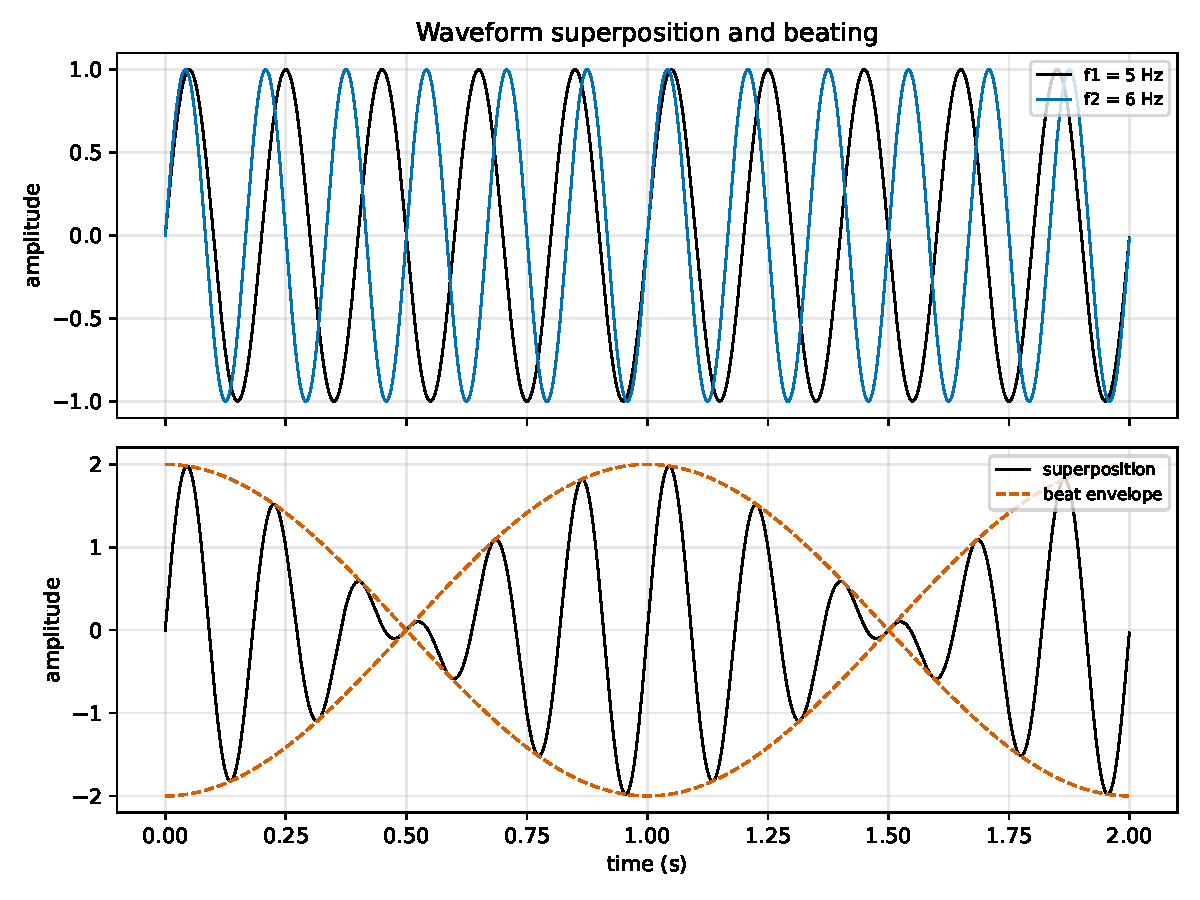
\includegraphics[width=0.85\linewidth]{figures/fig_wave_superposition.pdf}
\caption{Two sinusoidal components and their time-domain superposition. Nearby frequencies produce a slow beat
envelope; equal-frequency addition reduces to the exact phasor law of Lemma~1.}
\label{fig:wave}
\end{figure}

\section{Related Work}
\label{sec:related}

The lattice model sits in the lineage of the Kuramoto model of coupled phase oscillators~\cite{kuramoto1975}, whose
onset of synchronization and mean-field theory are surveyed by Strogatz~\cite{strogatz2000} and, comprehensively, by
Acebr\'on and colleagues~\cite{acebron2005}. Our departure is that couplings are signed by a geometric orientation
class and the polar class is antiferromagnetic, so the lattice is frustrated: not all pairwise alignment preferences
can be satisfied at once. Frustration in this precise sense goes back to Villain's analysis of competing
interactions and spin glasses~\cite{villain1977}, and it is the mechanism that keeps the phase field in the
partially ordered regime of Section~\ref{sec:latticeresults} rather than at global lock.

The SCM is a coupled dynamical network on a ring and is close in spirit to Kaneko's coupled map
lattices~\cite{kaneko1992}, which showed that simple local maps with diffusive coupling generate rich spatiotemporal
behavior. The term \emph{stable chaos} is due to Politi and Torcini~\cite{politi2010}, who reserve it for irregular
dynamics in linearly stable systems; we adopt it operationally, as stated in Section~\ref{sec:intro}, without
claiming to have measured Lyapunov exponents. Finally, the SCM's two-channel, opposition-plus-noise design was
motivated in part as a response to probabilistic-bit (p-bit) computing~\cite{camsari2019}, which builds computation
from stochastic binary units; the SCM instead keeps a bounded continuous state and studies the persistence and
occupancy that antagonistic and imitative coupling produce together.

\section{Discussion and Future Work}
\label{sec:discussion}

The two models support a single, deliberately modest claim: antagonistic and imitative coupling, each impoverished
on its own, together sustain bounded, non-converging dynamics that remain both persistently mobile and cross-node
diverse. As the ablations show, occupancy entropy alone does not certify this, since an unanchored herd also visits
much of the space; the operational signature is instead the conjunction of liveness and diversity. We have stated this
operationally and backed it with reproducible, seed-controlled figures and metrics; the SCM ablations isolate the
two mechanisms, and the lattice sweep isolates frustration. We emphasize the scope. This is a computational
exploration of finite discrete and semi-discrete models. We do not take a continuum limit, we do not estimate
Lyapunov spectra, and we make no hardware claims; the ``chaos'' in our title is the operational notion of
Section~\ref{sec:intro}, aligned in spirit with but not a measurement of the stable chaos of~\cite{politi2010}.

Several extensions follow directly from the constructions. The orientation classifier and the lattice already
support the toroidal option and dimensions one through three, so the frustrated phase dynamics can be studied on
higher-dimensional tori where every node has the full $6/12/8$ neighborhood and boundary effects vanish. The exact
phasor algebra of Section~\ref{sec:waves} invites an audio reading of the lattice, mapping node phases to partials
and studying the timbral consequences of frustration, and the same orientation-classed couplings suggest a
constraint-driven, wave-function-collapse style of spatial generation. Quantifying the SCM's persistence spectrally
through the autocorrelation of Section~\ref{sec:metrics}, and mapping the full $(N,\delta)$ parameter surface, are
the natural next measurements. Each of these is a concrete, testable continuation of the same thesis: opposition
without imitation freezes, imitation without opposition collapses, and the two together stay alive.

\begin{thebibliography}{9}

\bibitem{kuramoto1975}
Y.~Kuramoto,
``Self-entrainment of a population of coupled non-linear oscillators,''
in \emph{International Symposium on Mathematical Problems in Theoretical Physics},
Lecture Notes in Physics, vol.~39, H.~Araki, Ed.
Berlin: Springer, 1975, pp.~420--422.

\bibitem{strogatz2000}
S.~H.~Strogatz,
``From Kuramoto to Crawford: exploring the onset of synchronization in populations of coupled oscillators,''
\emph{Physica D}, vol.~143, no.~1--4, pp.~1--20, 2000.

\bibitem{acebron2005}
J.~A.~Acebr\'on, L.~L.~Bonilla, C.~J.~P\'erez Vicente, F.~Ritort, and R.~Spigler,
``The Kuramoto model: a simple paradigm for synchronization phenomena,''
\emph{Reviews of Modern Physics}, vol.~77, no.~1, pp.~137--185, 2005.

\bibitem{kaneko1992}
K.~Kaneko,
``Overview of coupled map lattices,''
\emph{Chaos}, vol.~2, no.~3, pp.~279--282, 1992.

\bibitem{politi2010}
A.~Politi and A.~Torcini,
``Stable chaos,''
in \emph{Nonlinear Dynamics and Chaos: Advances and Perspectives}, Understanding Complex Systems.
Berlin: Springer, 2010, pp.~103--129.

\bibitem{camsari2019}
K.~Y.~Camsari, B.~M.~Sutton, and S.~Datta,
``p-bits for probabilistic spin logic,''
\emph{Applied Physics Reviews}, vol.~6, no.~1, art.~011305, 2019.

\bibitem{villain1977}
J.~Villain,
``Spin glass with non-random interactions,''
\emph{Journal of Physics C: Solid State Physics}, vol.~10, no.~10, pp.~1717--1734, 1977.

\end{thebibliography}

\end{document}
